\section{Quadratic Functions}

    \subsection{Miscellaneous Quadratic Info}
        %Table with three forms of quadratic function
        \begin{center}
            \begin{tabular}{|c|c|}
                \hline
                $ax^2+bx+c$   & Standard Form  \\
                \hline
                $a(x-h)^2+k$  & Vertex Form    \\
                \hline
                $a(x-p)(x-q)$ & Intercept Form \\
                \hline
            \end{tabular}
        \end{center}

        \noindent The vertex is given by $(h,k)$, where $h=-\frac{b}{2a}$. The roots are given
        by $p$ and $q$. The intercept form is also known as the factored form. The
        \textbf{axis of symmetry} which divides a quadratic graph into right and left sides,
        is given by the line $x=-\frac{b}{2a}$.



    \subsection{Graphing Quadratic Functions}
        1. Find the vertex \\
        2. Find the $y$-intercept \\
        3. Find the $x$-intercept(s) \\
        4. Test two points minimum, one on each side of the vertex. \\
        5. Connect the points.

        % Graph of quadratic parent function
        \begin{center}
            \begin{tikzpicture}
                \begin{axis} [
                    axis lines = center,
                    xlabel = {$x$},
                    ylabel = {$y$},
                    xmajorticks=false,
                    ymajorticks=false
                ]
                %%%
                \addplot [
                    domain = -20:20,
                    samples = 40,
                    color = red
                ]
                {x^2};
                \addlegendentry{$y=x^2$}
                \end{axis}
            \end{tikzpicture}
        \end{center}



    \subsection{Factorization}
        \textbf{The Four Common Methods of Factoring:} \\
        \color{purple} \textbf{1. Greatest Common Factor} \color{black} \\
        $a(b+c)=ab+ac$ \\
        \color{purple} \textbf{2. Grouping} \color{black} \\
        This method is typically done with a four-term polynomial. Group the first two terms
        and the last two terms, then factor out a GCF from the two groups, and combine like
        polynomials. When the polynomial only has three terms, we can manipulate it so that the
        polynomial gains another term. We do this by multiplying the general quadratic
        coefficients $a$ and $c$ and then finding two factors of $ac$ which have a sum equal to
        the middle term's general coefficient, $b$. \\

        \noindent \color{blue} \textit{Example 1: Factor $x^3+7x^2+2x+14$} \color{black} \\
        \begin{align*}
            x^3+7x^2+2x+14 &= (x^3+7x^2) + (2x+14) \\
            &= (x^2(x+7) + 2(x+7)) \\
            &= (x+7)(x^2+2)
        \end{align*}

        \noindent \color{blue} \textit{Example 2: Factor $x^5-3x^3-2x^2+6$} \color{black} \\
        \begin{align*}
            x^5-3x^3-2x^2+6 &= (x^5-3x^3) - (2x^2-6) \\
            &= x^3(x^2-3) - 2(x^2-3) \\
            &= (x^2-3)(x^3-2)
        \end{align*}

        \noindent \color{blue} \textit{Example 3: Factor $3x^2+2x-8$} \color{black} \\
        The product $ac$ is given by $(3)(-8) = -24$. Its factors -4 and 6 have a sum of 2
        which is equal to $b$, the coefficient of the middle term. Thus, we can split the $2x$
        into two terms as below.

        \begin{align*}
            3x^2+\color{blue}2x\color{black}-8 &= 3x^2\color{blue}-4x+6x\color{black}-8 \\
            &= (3x^2-4x) + (6x-8) \\
            &= x(3x-4) + 2(3x-4) \\
            &= (3x-4)(x+2)
        \end{align*}

        \pagebreak
        \noindent \color{blue} \textit{Example 4: Factor $4x^2+10x-6$} \color{black} \\
        Again, the product $ac$ is given by $(4)(-6) = -24$. Its factors -2 and 12 have a sum
        of $b=10$. Thus, it can be factored by grouping:

        \begin{align*}
            4x^2+\color{blue}10x\color{black}-6 &= 4x^2\color{blue}-2x+12x\color{black}-6 \\
            &= (4x^2-2x) + (12x-6) \\
            &= 2x(2x-1) + 6(2x-1) \\
            &= (2x+6)(2x-1)
        \end{align*}

        \noindent \color{purple} \textbf{Special Forms:} \color{black} \\
        For factoring higher-degree polynomials, simply employ the usual methods of
        factorization. Below are some general factorizations that should be memorized.

        %Sum/Difference of Squares and Cubes
        \begin{center}
            \begin{tabular}{|c|c|}
                \hline
                $(a\pm b)^2 = a^2\pm 2ab+b^2$         & \textbf{Sum/Difference of Perfect Squares} \\
                \hline
                $a^2-b^2=(a+b)(a-b)$                  & \textbf{Difference of Squares}             \\
                \hline
                $a^3\pm b^3=(a\pm b)(a^2 \mp ab+b^2)$ & \textbf{Sum/Difference of Cubes}           \\
                \hline
            \end{tabular}
        \end{center}



    \subsection{Completing the Square}
        Taking a quadratic equation of the form $ax^2+bx+c=0$, completing the square allows us to
        rewrite this equation as $a(x+d)^2+e=0$, where $d=\frac{b}{2a}$ and $e=c-\frac{b^2}{4a}$.
        This method was inspired by the geometric representation of $x^2+bx$ being completed by
        $\left(\frac{b}{2}\right)^2$.

        \begin{figure} [hbt!]
            \centering
            \includegraphics [scale = 0.4] {Resources/Unit2Quadratics/Completing_The_Square.png}
        \end{figure}

        \noindent \color{blue} \textit{Example: Complete the square for $x^2+4x+1$} \color{black} \\
        $\left(\frac{b}{2}\right)^2 = 4$, so we add 4 and subtract 4. Parantheses are added to
        better conceptualize the later simplification.

        \begin{align*}
            (x^2+4x+4)+1-4 &= (x^2+4x+4) - 3 \\
            &= (x+2)^2 - 3
        \end{align*}



    \subsection{The Loh Method}
        Originally devised by ancient Babylonians and Greeks, this method was revised by Viete
        and rediscovered by Professor Po-Shen Loh in late 2019. We will refer to this as the
        Loh Method for ease of explanation. \\

        \noindent \color{blue} \textit{Example 1: Solve $x^2-14x+24=0$} \color{black} \\
        The factorization will be in the form $(x-\longunderscore)(x-\longunderscore)$.
        The method says that \textit{if and only if} we can find two numbers such that their sum
        is the opposite of $b$, in this case 14, and their product is $c$ which is 24 in this case
        then those numbers are the solutions. This method is an extremely convenient way of finding
        the solutions for \textit{any} quadratic equation, even irrational ones that would be hard
        to guess. \\

        \noindent This method uses the concept that our two numbers that add to 14 have an average
        of 7, since $\frac{14}{2} = 7$. Taking the average of two numbers, we know that one of the
        factors will be a little smaller than 7 and the other factor will be a little greater than
        7. We can express the smaller factor by "7-$u$" and the greater factor by "7+$u$". We know
        that the factors have a product of 24, thus

        \begin{align*}
            24  &= (7-u)(7+u) \\
            &= 49 - u^2 \\
            u^2 &= 25 \\
            u   &= \pm 5
        \end{align*}

        \noindent Since $u = \pm 5$ exists, we can calculate $7-u = 7-5 = 2$ and $7+u=7+5=12$.
        Using $u=-5$ would produce the same values. Now we plug 2 and 12 into
        $(x-\longunderscore)(x-\longunderscore)$, giving us

        \begin{align*}
            0          &= x^2-14x+24 \\
            &= (x-2)(x-12) \\
            \implies x &= 2,12
        \end{align*}

        \noindent Using other factorization methods, we verify that these are indeed the solutions
        to the quadratic equation. \\

        \noindent \color{blue} \textit{Example 2: Solve $x^2-8x+13=0$} \color{black} \\
        Using other methods, we would not have been able to factor this since 13 is a prime number.
        Again, $x^2-8x+13 = 0 = (x-\longunderscore)(x-\longunderscore)$. \\

        \noindent If we can find two numbers that have a sum of 8 and a product of 13, then they
        are the solutions. Looking at the product which is 13, it's very hard to think of factors
        of 13 which have a sum of 8. Once again, there are two numbers that have an average of 8,
        so we will need $u$ to satisfy the below equation.

        \begin{align*}
            13  &= (4-u)(4+u) \\
            &= 16 - u^2 \\
            u^2 &= 3 \\
            u   &= \pm \sqrt{3}
        \end{align*}

        \noindent We can ignore the negative value of $u$ since it will give the same values as its
        opposite. Thus, \\

        \begin{align*}
            0          &= x^2-8x+13 \\
            &= \left(x-[4-\sqrt{3}]\right) \left(x-[4+\sqrt{3}]\right) \\
            \implies x &= 4 \pm \sqrt{3}
        \end{align*}



    \subsection{The Quadratic Formula}
        We can derive the quadratic formula through completing the square. \\

        \begin{align*}
            ax^2+bx+c                                                                 &=  0 \\
            (ax^2+bx)+c                                                               &=  0 \\
            a\left(x^2+x\cdot\frac{b}{a}\right)+c                                     &= 0 \\
            a\left(x^2+x\cdot\frac{b}{a}+\frac{b^2}{4a^2}\right)+c-\frac{b^2}{4a^2}   &= 0 \\
            a\left(x^2+x\cdot\frac{b}{a}+\frac{b^2}{4a^2}\right)+c = \frac{b^2}{4a^2} &= \frac{b^2}{4a^2} \\
            a\left(x+\frac{b}{2a}\right)^2   &= \frac{b^2}{4a} - c \\
            \left(x+\frac{b}{2a}\right)^2   &= \frac{b^2}{4a^2} - \frac{c}{a} \\
            \left(x+\frac{b}{2a}\right)^2   &= \frac{b^2-4ac}{4a^2} \\
            x + \frac{b}{2a}                &= \pm\frac{\sqrt{b^2-4ac}}{2a}
        \end{align*}

        \begin{equation*}
            \bm{{x &= \frac{-b\pm\sqrt{b^2-4ac}}{2a}}}
        \end{equation*}



    \subsection{Imaginary and Complex Numbers}
        When a quadratic solution involves a negative number under a radicand, that solution is
        either imaginary or complex. Recall that pure imaginary numbers are of the form $bi$,
        where $i=\sqrt{-1}$ and complex numbers are of the form $a+bi$. \\

        \noindent \color{blue} \textit{Example 1: $x^2+4x+5=0$} \color{black} \\
        Using the quadratic formula, we compute $x$ to be \\

        \begin{align*}
            x &= \frac{-4\pm\sqrt{-4}}{2} \\
            &= \frac{-4\pm 2i}{2} \\
            &= -2 \pm i
        \end{align*}

        \noindent If we wanted to efficiently find the behavior of a quadratic's roots, we could use the
        \textbf{discriminant}, $b^2-4ac$. \\

        % Table describing relationship between discriminant and roots
        \begin{center}
            \color{purple} \textbf{Types of Roots} \color{black} \\
            %%%
            \begin{tabular}{|c|c|c|}
                \hline
                Discriminant is positive & Discriminant is zero   & Discriminant is negative   \\
                \hline
                $b^2-4ac>0$              & $b^2-4a=0$             & $b^2-4ac<0$                \\
                \hline
                \textit{Two Real Roots}  & \textit{One Real Root} & \textit{Two Complex Roots} \\
                \hline
            \end{tabular}
        \end{center}



    \subsection{Mathematical Modeling with Quadratic Functions}

        Quadratic functions are often used for modeling flying objects, for example the flight trajectory of a thrown
        ball. Consider the graph of $f(t) = -(t-3)^2+9$, where $t>0$. If $t$ represents time, then
        $f(t)$ represents the height at which the ball is at a particular time. We can then clearly
        see from the graph that the ball is at a height of 0 when time is 0. The ball reaches its peak
        height of 9 at the vertex of the quadratic function when time is 3, and descends to a height of
        0 at the second root of the function.

        \begin{center}
            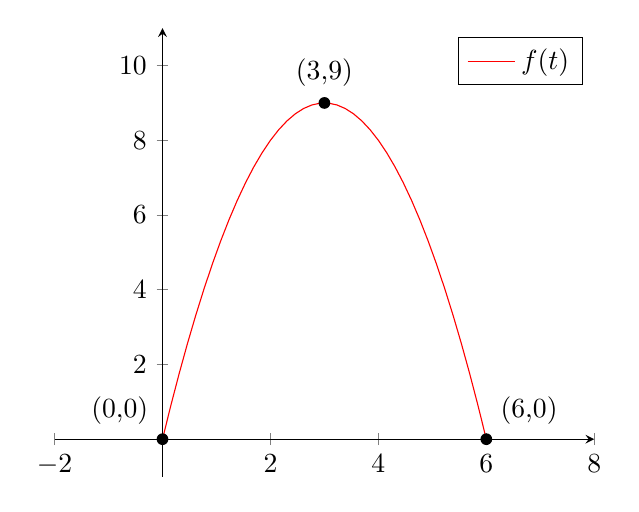
\begin{tikzpicture}
                \begin{axis} [
                    axis lines = center,
                    ymin = -1,
                    ymax = 11,
                    xmin = -2,
                    xmax = 8
                ]
                %%%
                \addplot [
                    domain = 0:6,
                    samples = 40,
                    color = red
                ]
                {-(x-3)^2+9};
                \addlegendentry{$f(t)$}
                %%%
                \node[label={135:{(0,0)}},circle,fill,inner sep=1.5pt] at (axis cs:0,0) {};
                \node[label={90:{(3,9)}},circle,fill,inner sep=1.5pt] at (axis cs:3,9) {};
                \node[label={45:{(6,0)}},circle,fill,inner sep=1.5pt] at (axis cs:6,0) {};
                \end{axis}
            \end{tikzpicture}
        \end{center}